% Mechanical Design Report - Sensor Box V2
\documentclass[12pt]{article}
\usepackage[margin=1in]{geometry}
\usepackage{graphicx}
\usepackage{caption}
\usepackage{float}

\title{Mechanical Design Report\\Sensor Box Iteration}
\author{0104C}
\date{\today}

\begin{document}

\maketitle

\section{Introduction}

This report documents the continued mechanical development of the sensor box, building on the rectangular enclosure and slidable lid concepts established in the 04.1.2 Mechanical Design Report. The design was refined to incorporate sensor-specific features and wiring access, and the first physical prints were used to validate the tolerance corrections from the previous iteration. Key design ideas carried forward successfully, but new fit issues were also encountered and resolved.

\section{Design Progress}

\subsection{Box V1: Added Features}

The initial rectangular profile from 04.1.2 was retained as the base geometry for Box V1. New features were added to address functional requirements that emerged from the integration work. A large circular opening was added to the front face to expose the sensor to the measurement environment. A grid of small ventilation holes was added to the lower front wall to allow airflow around the electronics. A circular side hole was also included to accommodate external connections. The slidable lid groove from 04.1.2 was carried forward at the top of the box. Figure \ref{fig:boxv1} shows the Box V1 CAD model.

\begin{figure}[H]
\centering
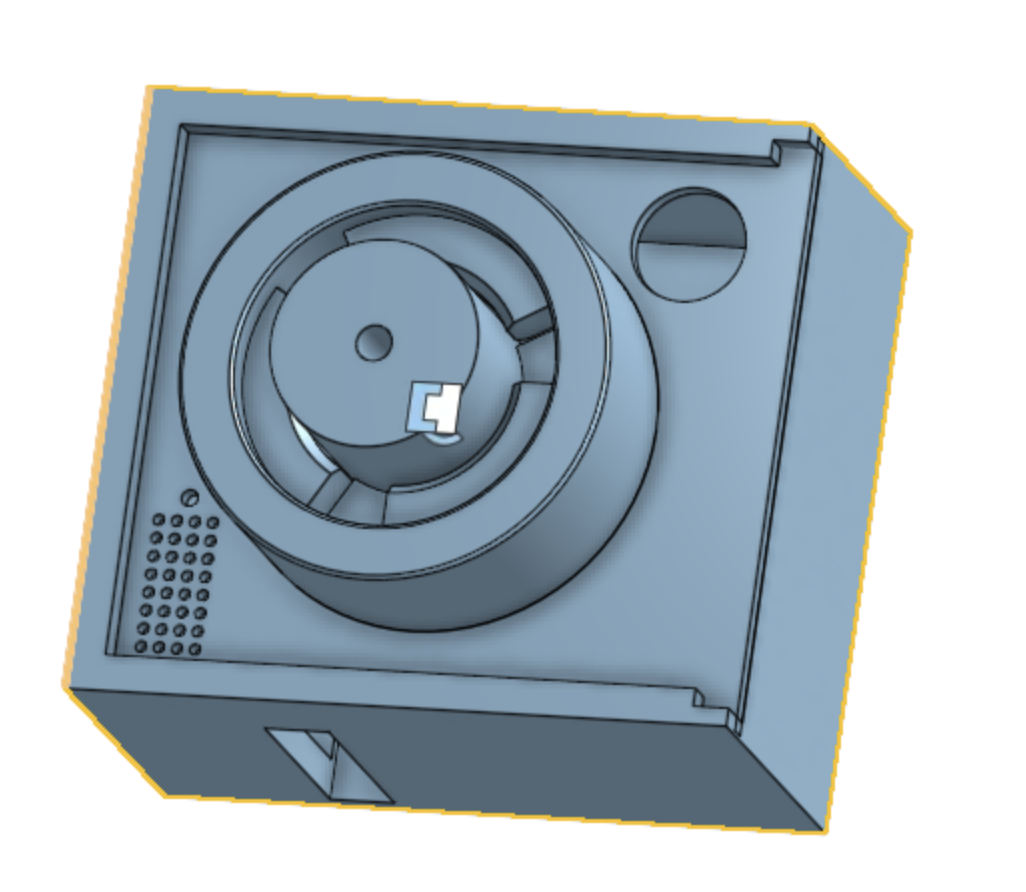
\includegraphics[width=0.70\textwidth]{images/Box V1.png}
\caption{Box V1 CAD model showing the sensor opening, ventilation holes, side hole, and slidable lid groove.}
\label{fig:boxv1}
\end{figure}

\subsection{Roof Tolerance Issue}

The first physical print of Box V1 reproduced the same fit problem identified in 04.1.2: the slidable lid was too wide to enter the groove on the box body. Figure \ref{fig:doesnotfit} shows the printed box and lid where the lid cannot be inserted. The CAD model had been updated with a small clearance gap following the 04.1.2 failure, but the gap was insufficient. A further increase to the clearance was applied to the model before reprinting.

\begin{figure}[H]
\centering
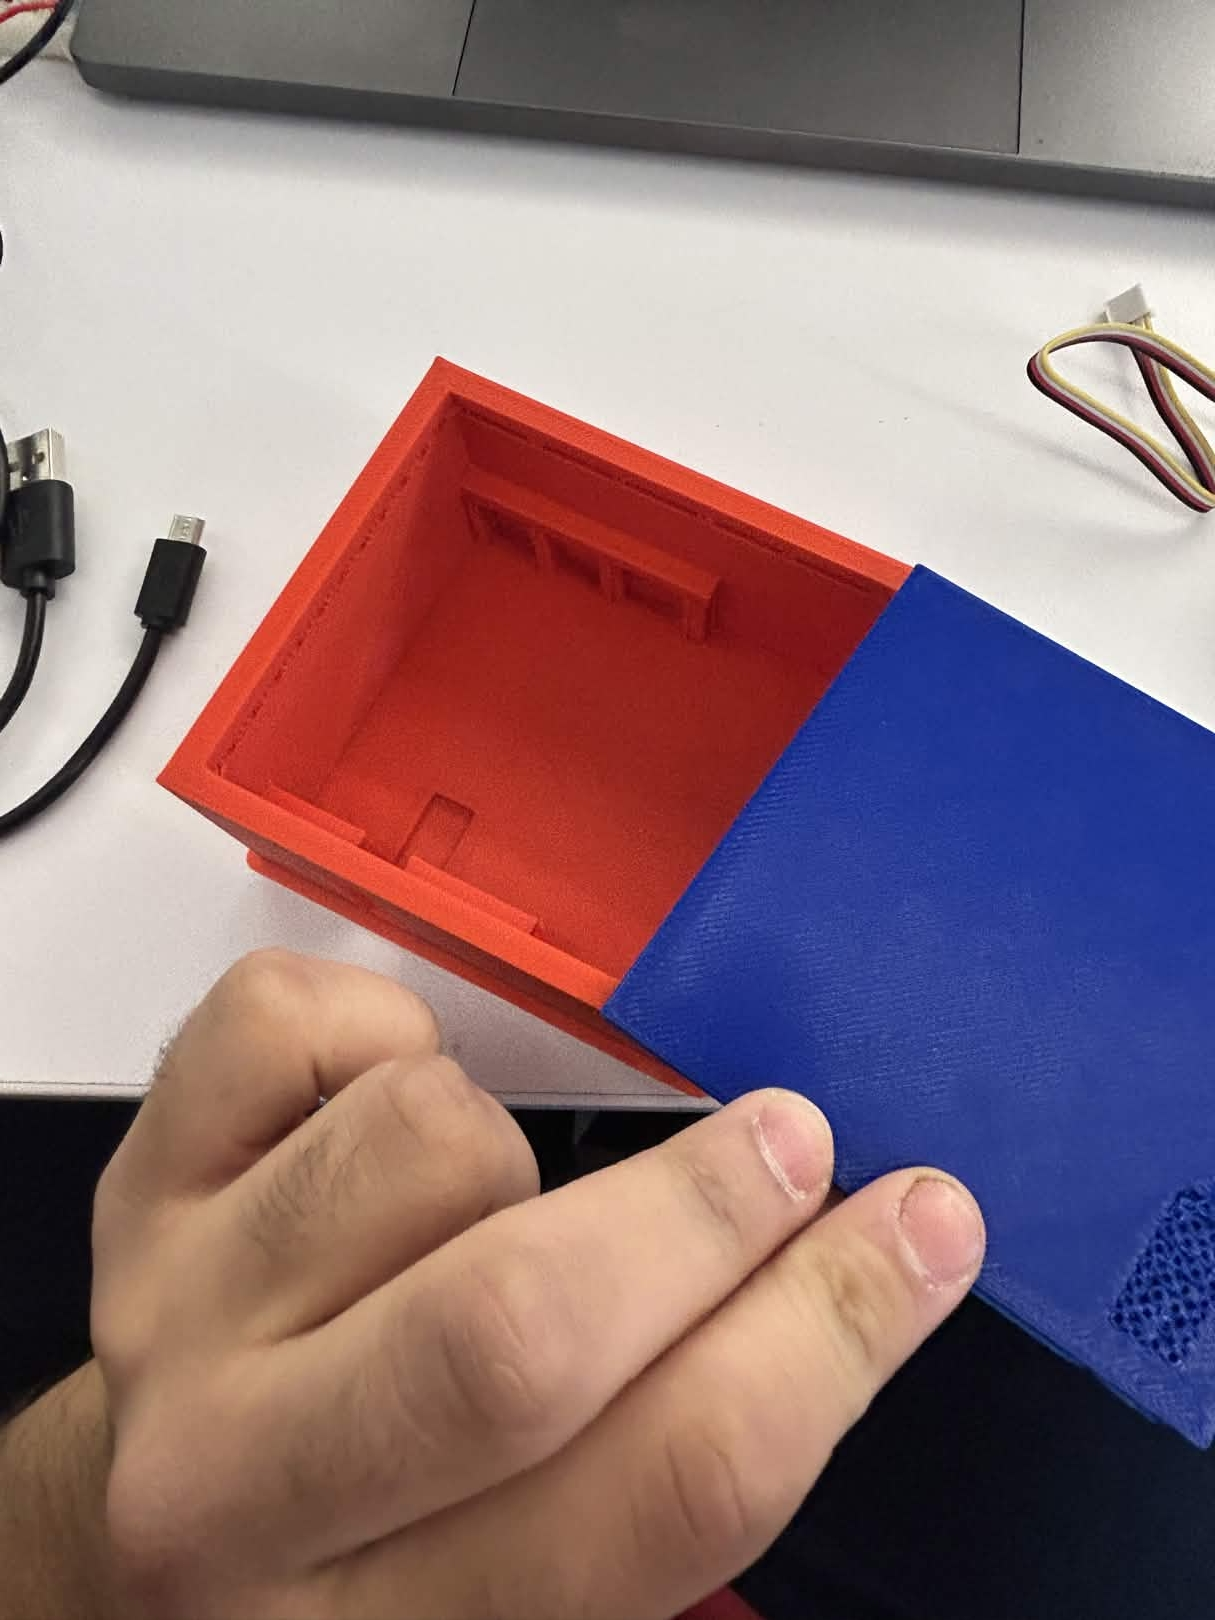
\includegraphics[width=0.65\textwidth]{images/Roof Does Not Fit.jpg}
\caption{First print of Box V1 showing the slidable lid unable to enter the box groove due to insufficient clearance.}
\label{fig:doesnotfit}
\end{figure}

\subsection{Wire Routing}

During assembly it became clear that jumper wires connecting the internal electronics to external components needed a dedicated exit point in the box wall. Small holes were introduced in the side panel to allow individual jumper wires to pass through cleanly without requiring the lid to be left open. Figure \ref{fig:wireholes} shows the wire routing holes in the panel.

\begin{figure}[H]
\centering
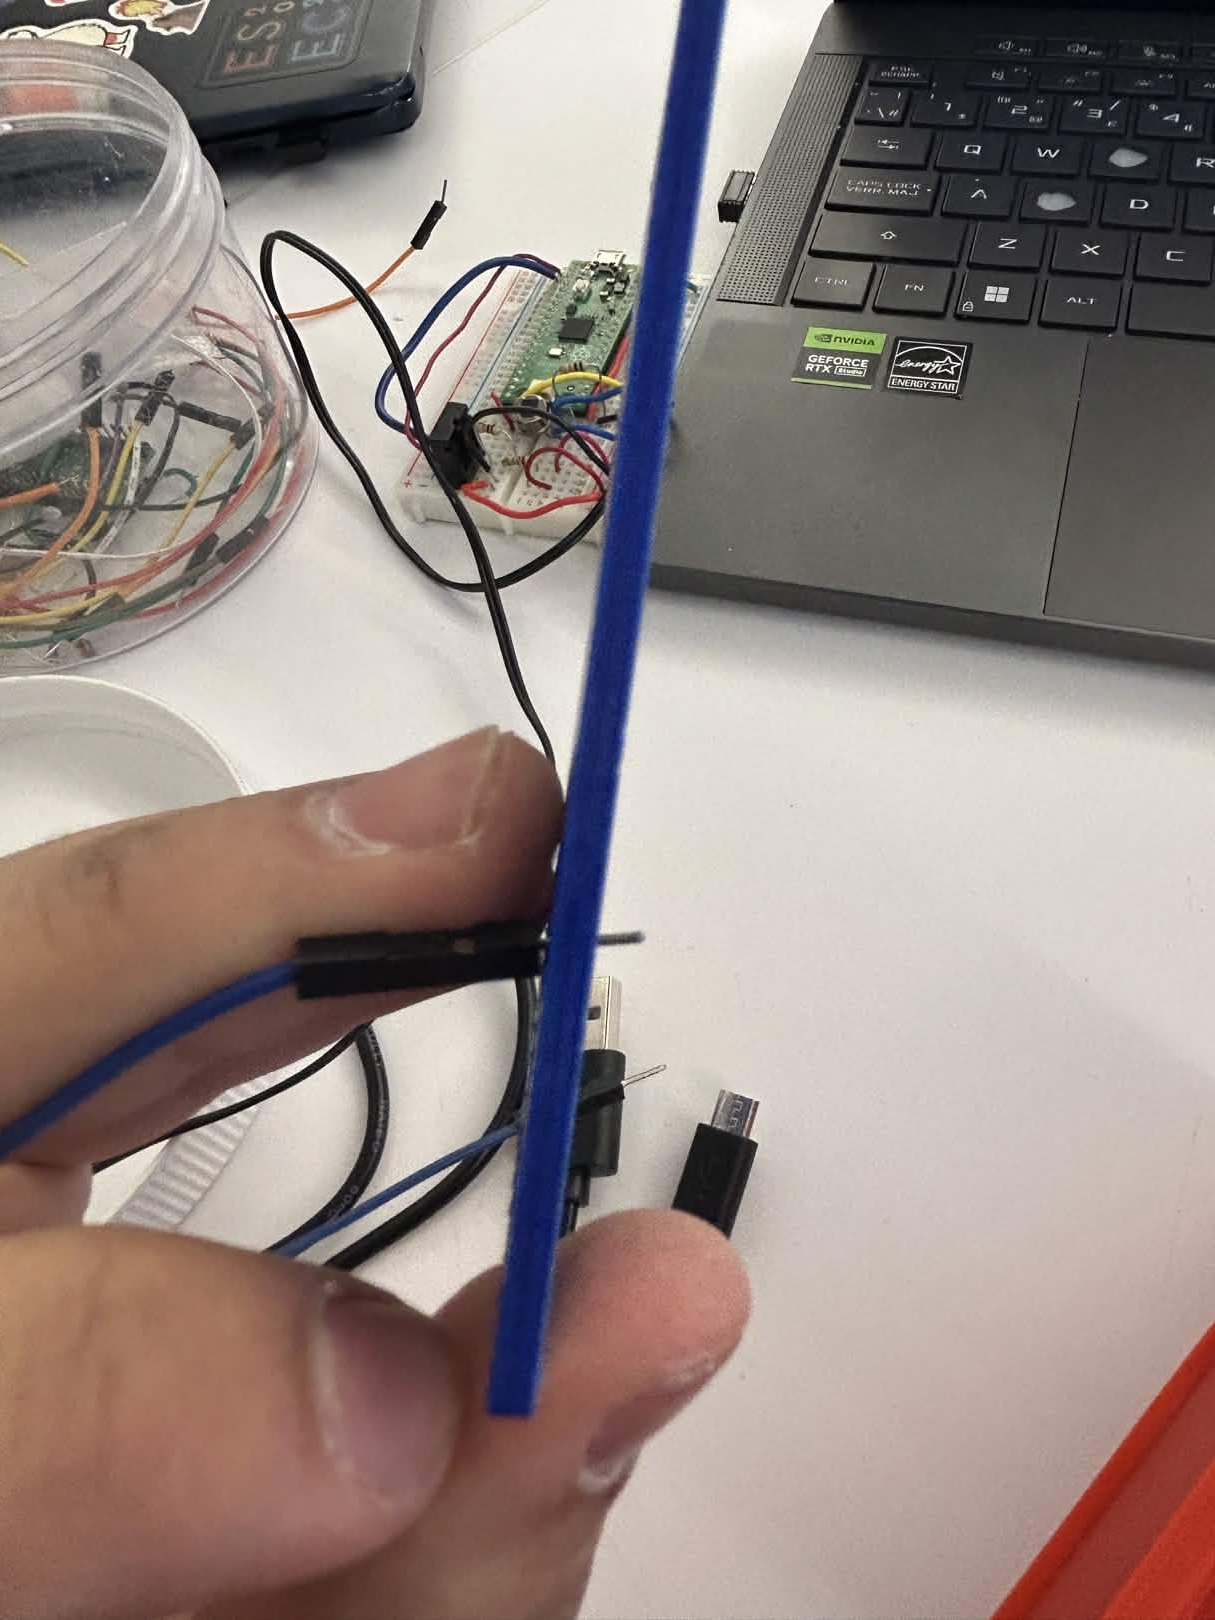
\includegraphics[width=0.65\textwidth]{images/Wire Holes for Jumpers.jpg}
\caption{Wire routing holes in the box panel allowing jumper wires to exit the enclosure.}
\label{fig:wireholes}
\end{figure}

\subsection{Side Access Slot}

A rectangular slot was also cut into the side of the box to provide additional access for connectors that could not pass through the smaller wire holes. Figure \ref{fig:sidehole} shows the side slot on the printed box.

\begin{figure}[H]
\centering
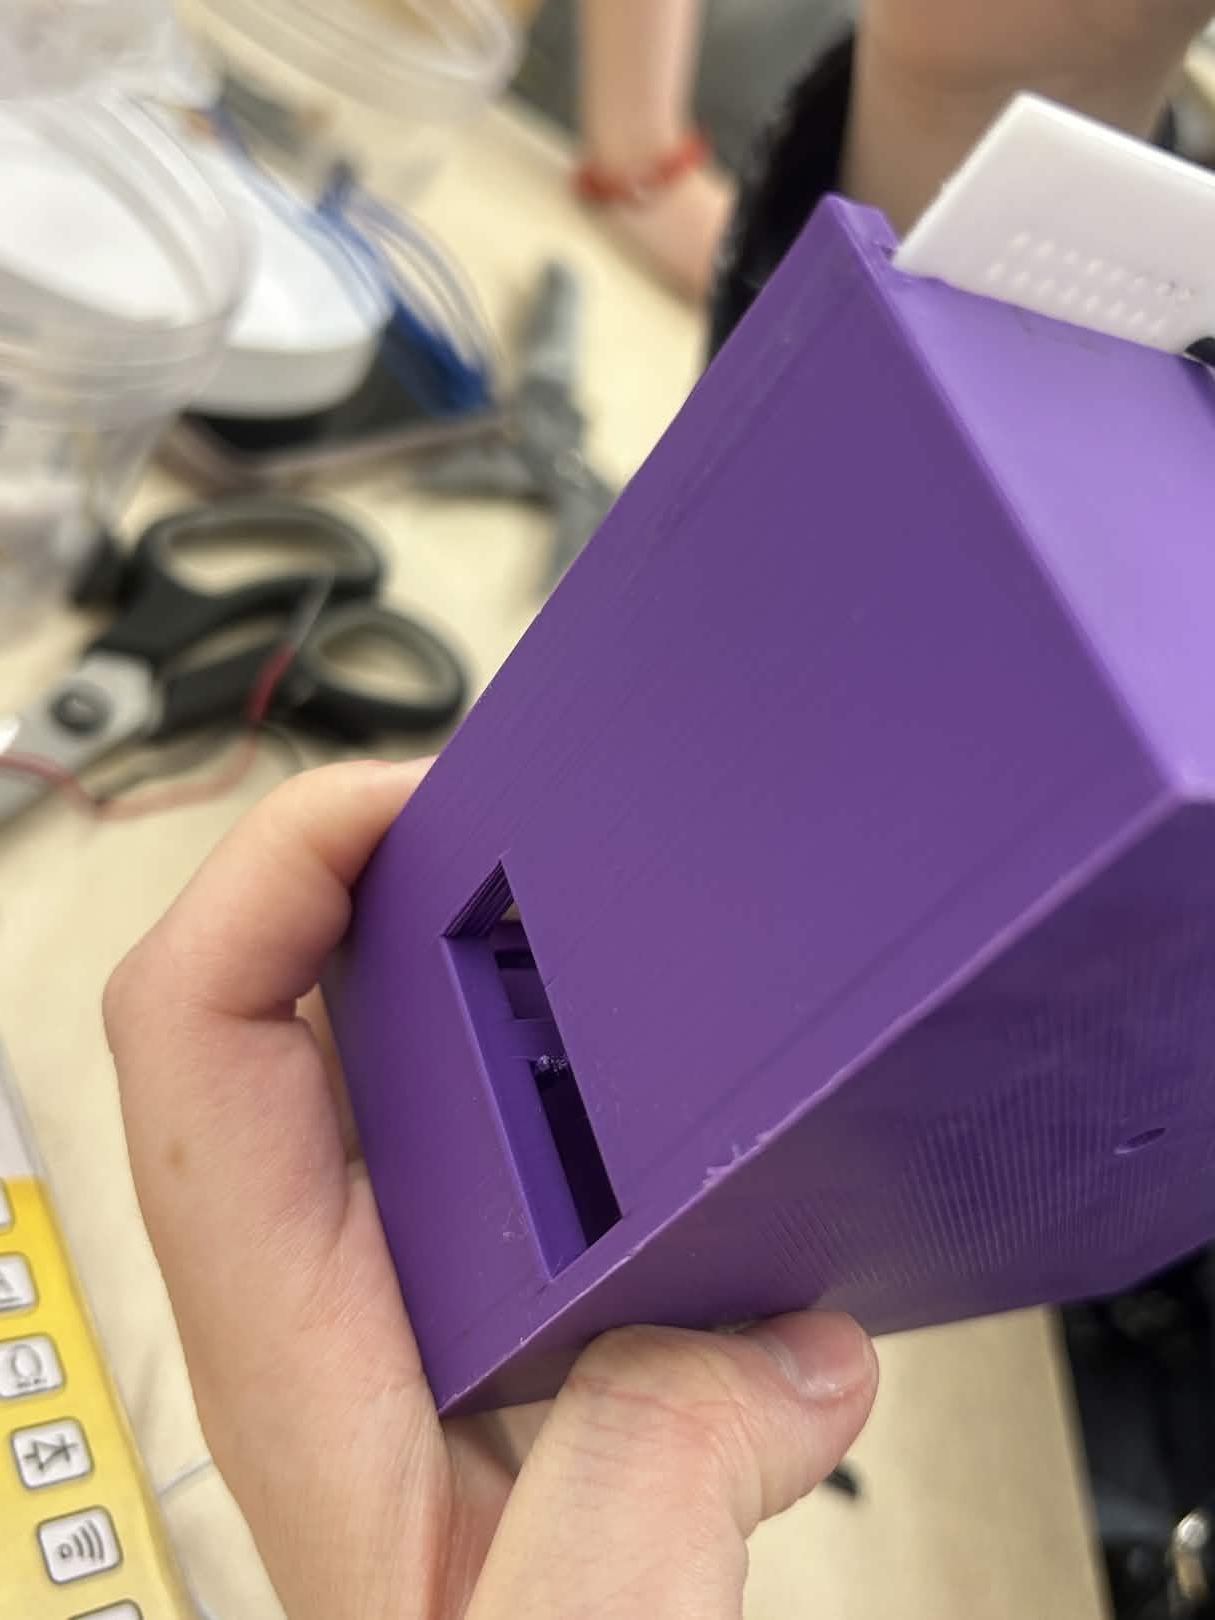
\includegraphics[width=0.65\textwidth]{images/Side Hole.jpg}
\caption{Rectangular access slot on the side of the box for connector routing.}
\label{fig:sidehole}
\end{figure}

\subsection{Roof Fit Resolved}

After increasing the clearance on the lid rail, a corrected print was produced. The slidable lid seated properly in the box groove and could be inserted and removed without resistance. Figure \ref{fig:rooffits} shows the corrected assembly with the lid in place.

\begin{figure}[H]
\centering
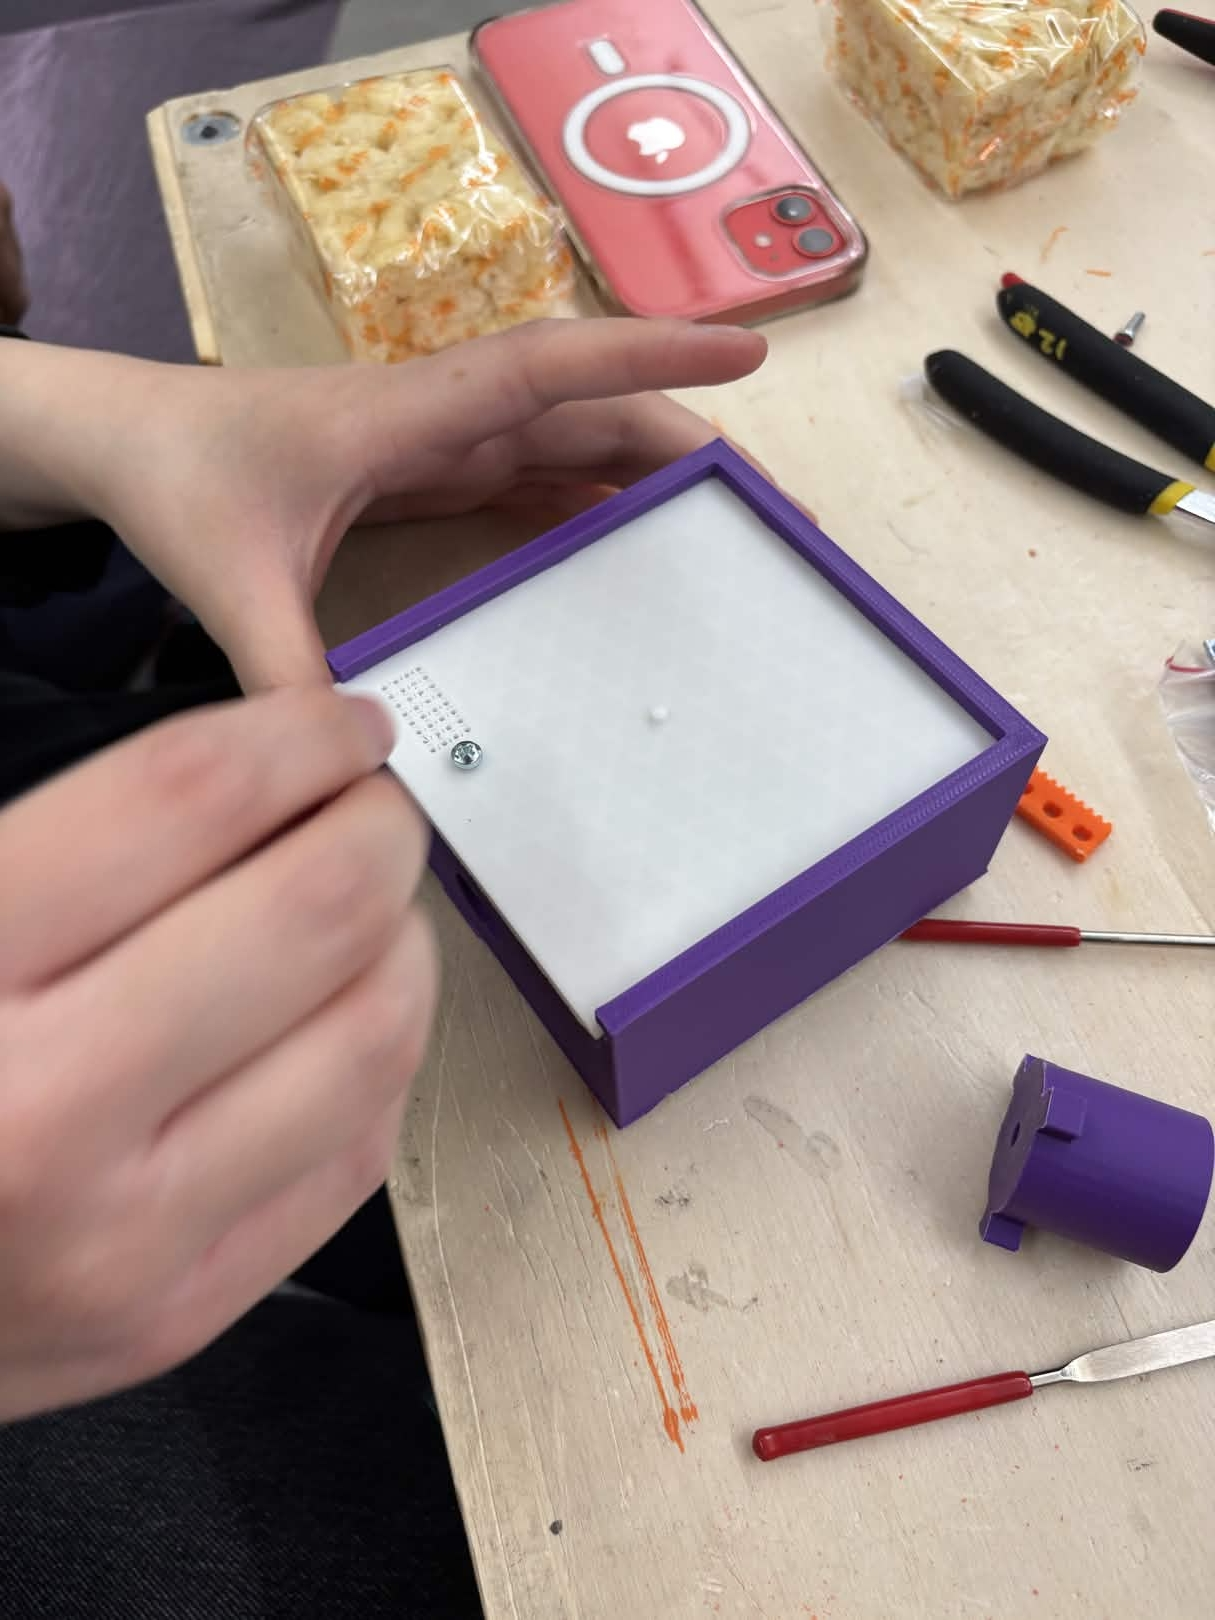
\includegraphics[width=0.65\textwidth]{images/Roof Fits.jpg}
\caption{Corrected print with the slidable lid fitting cleanly into the box groove.}
\label{fig:rooffits}
\end{figure}

\subsection{Final Box V2 Design}

With the fit issues resolved and the feature set confirmed, the design was consolidated into Box V2. The CAD model was cleaned up and the sensor mount was separated into a standalone cylindrical component to allow it to be printed and positioned independently. A cone piece was also included as a directional guide for the sensor opening. Figure \ref{fig:boxv2} shows the exploded view of the Final Box V2 assembly.

\begin{figure}[H]
\centering
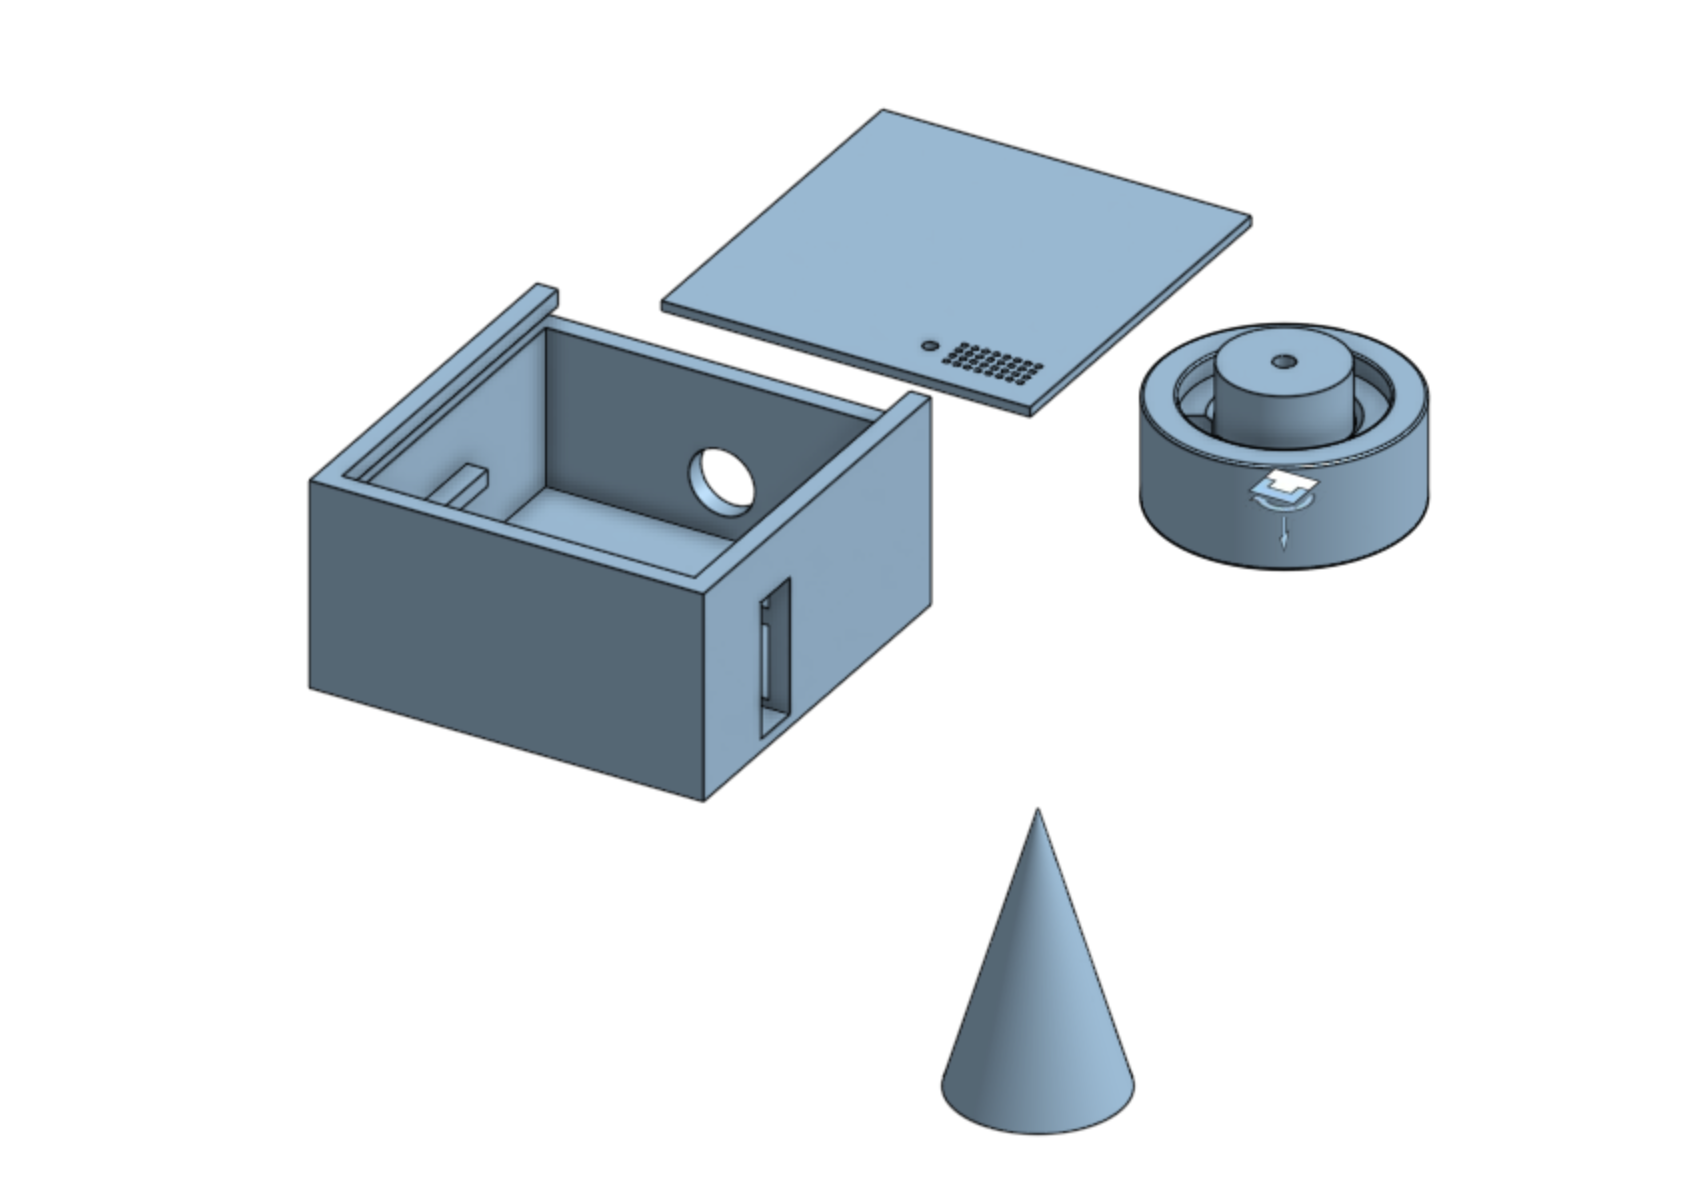
\includegraphics[width=0.70\textwidth]{images/Final Box V2.png}
\caption{Final Box V2 exploded CAD view showing the box body, slidable lid, cylindrical sensor mount, and cone guide.}
\label{fig:boxv2}
\end{figure}

\section{Conclusion}

The Box V1 design successfully evolved the initial concept from 04.1.2 by adding sensor-specific features including the front circular opening, ventilation holes, wire routing holes, and side access slot. The slidable lid concept was carried forward and the persistent tolerance issue from 04.1.2 was fully resolved after a second clearance adjustment. The design was then consolidated into Final Box V2 with a separate sensor mount component, producing a functional and printable enclosure for the sensor box deployment system.

\end{document}
